\documentclass[10pt]{beamer}

%%%
% PREAMBLE FOR THIS DOC 
%%%
%https://tex.stackexchange.com/questions/68821/is-it-possible-to-create-a-latex-preamble-header
\usepackage{/Users/miw267/Repos/csci246_spring2025/slides/preambles/beamer_preamble_for_CSCI246}



%%% TRY TO RESHOW TOC AT EACH SECTION START (with current section highlighted)
% Reference: https://tex.stackexchange.com/questions/280436/how-to-highlight-a-specific-section-in-beamer-toc
\newcommand\tocforsect[2]{%
  \begingroup
  \edef\safesection{\thesection}
  \setcounter{section}{#1}
  \tableofcontents[#2,currentsection]
  \setcounter{section}{\safesection}
  \endgroup
}


%%%% HERES HOW TO DO IT CORRECTLY
% FIRST IN .STY FILE, DO
%\usetheme[sectionpage=none]{metropolis}
% THEN AT EACH SECTION DO
%\begin{frame}{Outline}
%  \tableofcontents[currentsection]	
%\end{frame}



%\setbeamertemplate{navigation symbols}{}
%\setbeamertemplate{footline}[frame number]{}


%%%
% DOCUMENT
%%%

\begin{document}

%\maketitle

%% Title page frame
%\begin{frame}
%    \titlepage 
%\end{frame}





\title{02/28/2025: Partitions}
\author{CSCI 246: Discrete Structures}
\date{Textbook reference: Sec 16, Scheinerman}

\begin{frame}
    \titlepage 
\end{frame}


\begin{frame}
\footnotesize 
\begin{mygreenbox}[title=Graded Quiz Pickup]
Quizzes are in the front of the room, grouped into four bins (A-G, H-L, M-R, S-Z) by last name. The quizzes are upside down with your last name on the back. Come find yours before, during, or after class.  Only turn the quiz over if it's yours.
\end{mygreenbox} 
\vfill 

%\begin{myredbox}[title=Announcements]
%
%This Friday's problem quiz will cover relations (including equivalence relations) - see slide decks from 2/19, 2/24, and 2/26.  \\
%
%Next Friday's problem quiz will cover partitions and functions
%
%\end{myredbox}
%
%\vfill 


\begin{myyellowbox}[title=Today's Agenda]
\begin{itemize}
	\item Reading and problems quiz (15 mins)
	\item Mini-lecture ($\approx$ 15 mins)
%	%
%	\begin{itemize}
%	\footnotesize 
%	\item Review induction 
%	\end{itemize}
%	%
	\item Group exercises ($\approx$ 15 mins)
\end{itemize}

%	Rationale for group exercises: we got shortchanged on time last couple days, and I already did a lot of lectures, so I want you to practice. Next problems quiz will cover relations and functions: Hamkins and 
%	
\end{myyellowbox}
\vfill 

\end{frame}

\begin{frame}
 \begin{myredbox}[title=Reading Quiz (Partitions)]  
\begin{enumerate}
	\item Give an example of a partition of the set $\set{1,2,3,4,5,6}$.
	\item How many different ways are there to rearrange the letters in the word \texttt{AARDVARK}?
\end{enumerate}
\end{myredbox}
\vfill 
\begin{mygreenbox}[title=Problems Quiz (Relations)]
\begin{enumerate}
\item The property \textit{irreflexive} is not the same as being not reflexive.  Give an example of a relation on a set that is neither reflexive nor irreflexive.   (You may express your answer either as a set of ordered pairs or as a graph.) 
\item A relation $R$ is defined on $\mathbb{Z}$ by $a\,R\,b$ if $a+b$ is even.  Is $R$ an equivalence relation? If so, pick one of the 3 properties that all equivalence relations have and prove that $R$ has that property.  If not, prove that $R$ is not an equivalence relation. 	
\end{enumerate}

\end{mygreenbox}
\vfill 
%\textbf{Remark.} For intuition, note that $x \equiv y$ (mod $n$) if $x$ and $y$ have the same remainder after dividing by $n$.  For example, $6 \equiv 1$ (mod 5).
\end{frame}


\begin{frame}[standout]
Highlights from reading
\end{frame}

\begin{frame}{Partitions}

\begin{mygreenbox}[title=Definition]
Let $A$ be a set.  A \textbf{partition of} $A$ is a set of nonempty, pairwise disjoint sets whose union is $A$	
\end{mygreenbox}
\vfill 
\begin{myredbox}[title=Example]
Let $A = \set{1,2,3,4,5,6}$, and let
\[ \mathcal{P} = \bigg\{ \set{1,2}, \set{3}, \set{4,5,6} \bigg\} \]	

\vfill
\begin{figure}
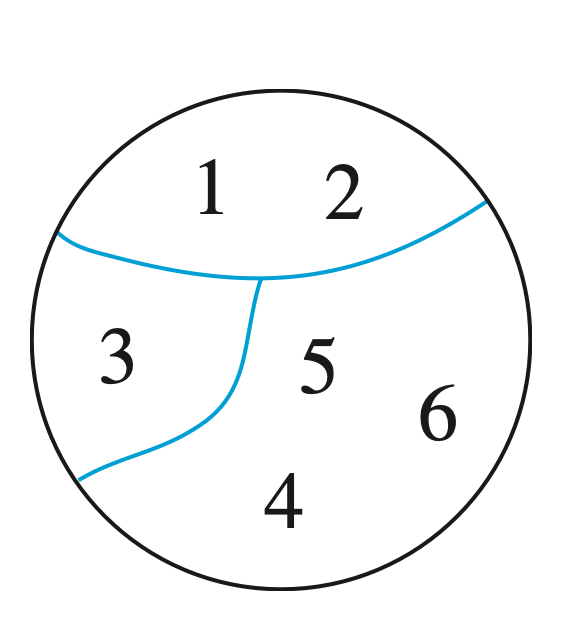
\includegraphics[width=0.2\textwidth]{images/partition.png}	
\end{figure}
\end{myredbox}

\end{frame}


\begin{frame}{From partitions to equivalence relations}
\footnotesize 
 \begin{mygreenbox}[title=Definition]  
Let $\mathcal{P}$ be a partition on a set $A$. The \textbf{is-in-the-same-part-as} relation, denoted  $\stackrel{\mathcal{P}}{=}$, is given by
\[ a \stackrel{\mathcal{P}}{=} b \quad  \iff \quad \exists P \in \mathcal{P} : a,b \in \mathcal{P} \]
\end{mygreenbox}
\vfill 
\begin{myyellowbox}[title=Remark]
In gist, we can take elements in the same cell to be related to each other. 
\end{myyellowbox}
\vfill 
\begin{myredbox}[title=Example]

\begin{minipage}{0.3\textwidth}

\begin{figure}
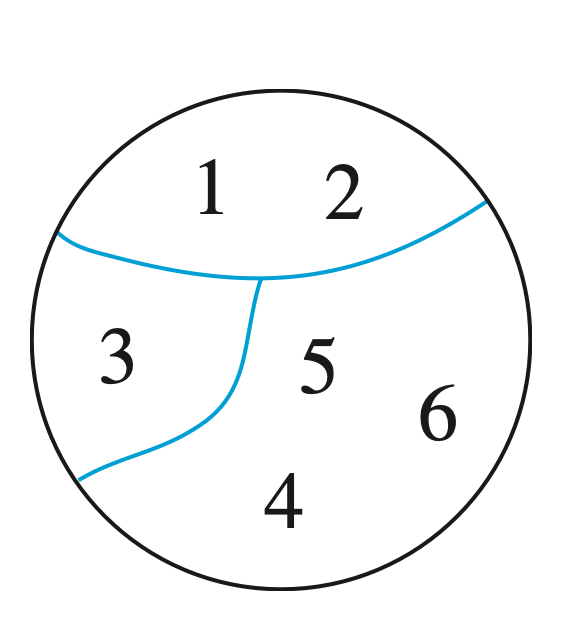
\includegraphics[width=0.5\textwidth]{images/partition.png}	
\end{figure}
\end{minipage}
\hfill 
\begin{minipage}{0.6\textwidth}
%For example, we have $1R2$ but $1 \cancel{R}3$.
The equivalence classes here are:
\begin{align*}
[1] &=  [2] = \set{1,2} \\
[3] &= \set{3} \\
[4] &= [5] = [6] = \set{4,5,6} 
\end{align*}
\end{minipage}
\end{myredbox}

\vfill 
 \begin{mygreenbox}[title=\text{Proposition (Scheinerman Prop 16.3)}]  
Let $\mathcal{P}$ be a partition on a set $A$. The relation $\stackrel{\mathcal{P}}{=}$ is an equivalence relation on $A$.
\end{mygreenbox}


\end{frame}

\begin{frame}{From equivalence relations to partitions}
\small 
 \begin{mygreenbox}[title=\text{Proposition (Scheinerman pp. 85)}]  
Let $R$ be an equivalence relation on $A$.  The equivalence classes of $R$ form a partition of the set $A$. 
\end{mygreenbox}
\vfill 
\begin{myredbox}[title=Example]
Setting $R$ to congruence mod 3, we can partition the integers into the following equivalence classes
%
\begin{align*}
[0] &= \set{\hdots, -6, -3, 0, 3, 6, \hdots} \\	
[1] &= \set{\hdots, -5, -2, 1, 4, 7, \hdots} \\	
[2] &= \set{\hdots, -4, -1, 2, 5, 8, \hdots} \\	
\end{align*}
\end{myredbox}

\end{frame}



\begin{frame}{Using equivalence relations to count}
\footnotesize 
 \begin{myyellowbox}[title=Question]  
How many ways are there to rearrange the letters in the word \texttt{HELLO}?
\end{myyellowbox}
\vfill 
 \begin{myredbox}[title=Solution]  
If there were no repeated letters (e.g. a big and small L), the answer would be $5!=120$.
%
\begin{figure}
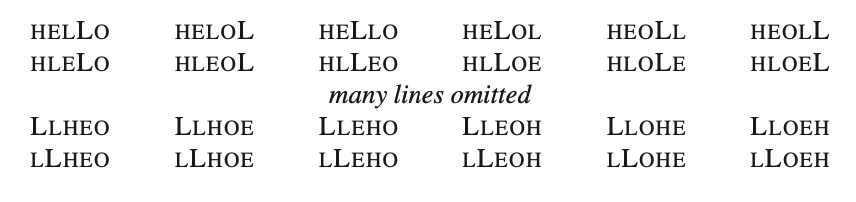
\includegraphics[width=0.5\textwidth]{images/hello}	
\end{figure}
%
But we must treat the big and small $L$ as equivalent.  We form equivalence classes, each of which have 2 members.
%
\begin{figure}
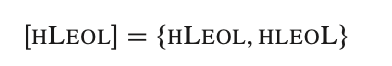
\includegraphics[width=0.5\textwidth]{images/hello_equiv}	
\end{figure}
%
All together there are $\frac{120}{2} = 60$ equivalence classes.  Hence, the answer is 120.
\end{myredbox}

\end{frame}

\begin{frame}
 \begin{mygreenbox}[title=\text{Theorem: Counting Equivalence Classes (Scheinerman Thm 16.6)}]  
Let $R$ be an equivalence relation on a finite set $A$. If all the equivalence classes of $R$ have the same size, $m$, then the number of equivalence classes is $|A|/m$. 
\end{mygreenbox}

\end{frame}


\begin{frame}[standout]
Feedback on Wednesday's Quiz 
\end{frame}



\begin{frame}{Scores On Reading Quiz (Equivalence Relations)(Extra Credit)}
\footnotesize 
\begin{figure}[ht]
        \centering
        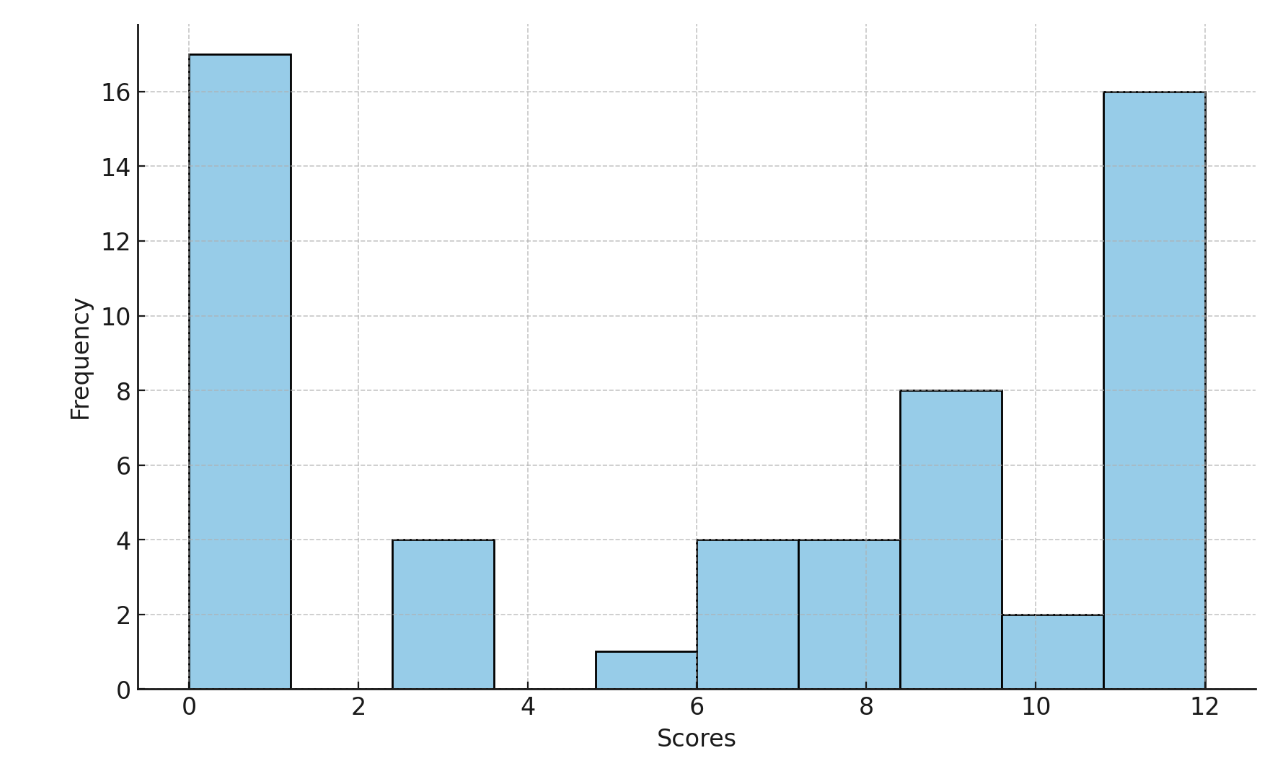
\includegraphics[width=.7\textwidth]{images/reading_quiz_scores}
   		 \caption{Median Score = 8/12 Extra Credit Points}
\end{figure}
\vfill 
\textbf{Rubric.}  	
\begin{itemize}
\item 3 points: Name the 3 properties of equivalence relation
\item For each of the 3 properties:
\begin{itemize} \footnotesize 
\item 1 point: Write out the property (or imply it)
\item 2 points: Prove that it holds
\end{itemize}
\end{itemize}
\end{frame}

\begin{frame}[standout]
Relation properties as pictures
\end{frame}

\begin{frame}[standout]
Group exercises
\end{frame}

\begin{frame}
\footnotesize 
\vfill 
\begin{columns}
\begin{column}{0.33\textwidth}
aaron.loomis: 8 \\ 
adam.wyszynski: 17 \\ 
alexander.goetz: 16 \\ 
alexander.knutson: 1 \\ 
anthony.mann: 15 \\ 
blake.leone: 5 \\ 
bridger.voss: 3 \\ 
caitlin.hermanson: 3 \\ 
cameron.wittrock: 10 \\ 
carsten.brooks: 13 \\ 
carver.wambold: 4 \\ 
colter.huber: 2 \\ 
conner.reed1: 4 \\ 
connor.mizner: 6 \\ 
connor.yetter: 2 \\ 
derek.price4: 19 \\ 
devon.maurer: 3 \\ 
emmeri.grooms: 4 \\ 
erik.moore3: 11 \\ 
ethan.johnson18: 15 \\ 
evan.barth: 19 \\\end{column}
\begin{column}{0.33\textwidth}
evan.schoening: 20 \\ 
griffin.short: 13 \\ 
jack.fry: 6 \\ 
jacob.ketola: 7 \\ 
jacob.ruiz1: 21 \\ 
jacob.shepherd1: 10 \\ 
jada.zorn: 10 \\ 
jakob.kominsky: 5 \\ 
james.brubaker: 18 \\ 
jeremiah.mackey: 9 \\ 
jett.girard: 9 \\ 
john.fotheringham: 7 \\ 
jonas.zeiler: 13 \\ 
joseph.mergenthaler: 21 \\ 
joseph.triem: 15 \\ 
julia.larsen: 17 \\ 
justice.mosso: 16 \\ 
kaden.price: 21 \\ 
lucas.jones6: 14 \\ 
luka.derry: 20 \\ 
luke.donaldson1: 6 \\\end{column}
\begin{column}{0.33\textwidth}
lynsey.read: 14 \\ 
mason.barnocky: 17 \\ 
matthew.nagel: 18 \\ 
micaylyn.parker: 19 \\ 
michael.oswald: 14 \\ 
nolan.scott1: 12 \\ 
owen.obrien: 1 \\ 
pendleton.johnston: 9 \\ 
peter.buckley1: 1 \\ 
reid.pickert: 5 \\ 
ryan.barrett2: 8 \\ 
samuel.hemmen: 2 \\ 
samuel.mosier: 18 \\ 
samuel.rollins: 12 \\ 
sarah.periolat: 12 \\ 
timothy.true: 8 \\ 
tristan.nogacki: 20 \\ 
tyler.broesel: 11 \\ 
william.elder1: 11 \\ 
yebin.wallace: 7 \\ 
zeke.baumann: 16 \\\end{column}
\end{columns}
\vfill
\end{frame}


\begin{frame}{Group exercises}
\footnotesize 

\begin{minipage}{0.66\textwidth}
\begin{enumerate}
\item How many different anagrams (including nonsensical words) can be made from each of the following? (a) \texttt{STAPLE}, (b)  \texttt{SUCCESS}, (c) \texttt{MISSISSIPPI}.
\item The integers 1 through 25 are arranged in a 5x5 array (we use each number from 1 to 25 exactly once). All that matters is which numbers are in which column and how they are arranged in the columns.  It does not matter in what order the columns appear. (See the figure.  The two arrays shown should be considered the same.) How many different such arrays can be formed?
\item Twelve people join hands for a circle dance. 
(a) In how many different ways can they do this? (b) Suppose six of these people are men, and the other six are women. In how many different ways can they join hands for a circle dance, assuming they alternate in gender around the circle?
\end{enumerate}
\end{minipage}
\hfill 
\begin{minipage}{0.31\textwidth}
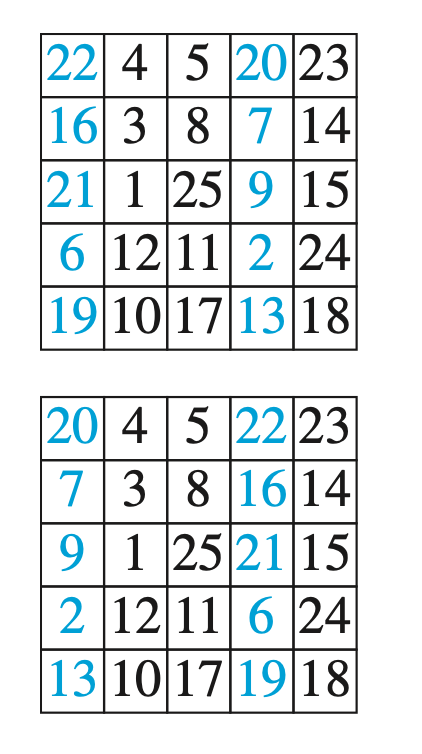
\includegraphics[width=0.7\textwidth]{images/partition_group_exercise.png}	
\end{minipage}
\end{frame}


\begin{frame}{Solution to group exercise \#1}
\textbf{Problem.} How many different anagrams (including nonsensical words) can be made from each of the following? (a) \texttt{STAPLE}, (b)  \texttt{SUCCESS}, (c) \texttt{MISSISSIPPI}.
\vfill 
\textbf{Solution.}

\begin{itemize}
\item[a.] $6!$. \quad  \textit{Justification}:  This is a simple permutation.  There are 6 choices for the first letter, 5 choices for the second letter, and so forth. We have done counting problems like this earlier in the course.  See Scheinerman Theorem 8.2 and/or Theorem 8.6.    
\item[b.] $\frac{7!}{2!3!}$. \quad  \textit{Justification:}  The number of ways to permute 7 distinct items is 7!, by the same logic as in part (a).  However, there are 3 S's, and rearrangements of those letters lead to an equivalent anagram.  Similarly for the 2 C's.  Hence, the solution follows from Scheinerman Theorem 16.6. 
\item [c.] $\frac{11!}{4!4!2!}$.  \quad  \textit{Justification:} The justification is similar as to that in part (b.)
\end{itemize}
\end{frame}


\begin{frame}{Solution to group exercise \#2}
\begin{minipage}{0.66\textwidth}
\textbf{Problem.} The integers 1 through 25 are arranged in a 5x5 array (we use each number from 1 to 25 exactly once). All that matters is which numbers are in which column and how they are arranged in the columns.  It does not matter in what order the columns appear. (See the figure.  The two arrays shown should be considered the same.) How many different such arrays can be formed?\\
\vfill 
\textbf{Solution.} There are $25!$ different ways to fill out the grid, by the same logic as in Problem 1a.  Once a grid layout is determined, there are $5!$ ways to rearrange the columns, all of which are to be considered equivalent. Hence, the number of distinct solutions is $\frac{25!}{5!}$, by Scheinerman Theorem 16.6.
\end{minipage}
\hfill 
\begin{minipage}{0.31\textwidth}
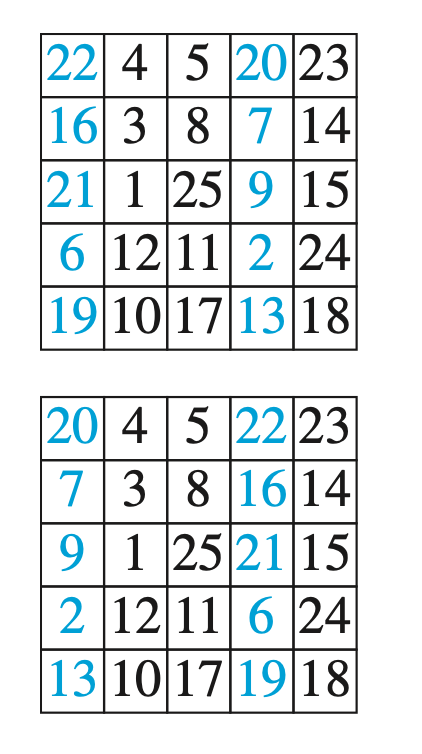
\includegraphics[width=0.7\textwidth]{images/partition_group_exercise.png}	
\end{minipage}
\end{frame}

\begin{frame}{Solution to group exercise \#3}
\scriptsize 
\textbf{Problem.} Twelve people join hands for a circle dance. 
(a) In how many different ways can they do this? (b) Suppose six of these people are men, and the other six are women. In how many different ways can they join hands for a circle dance, assuming they alternate in gender around the circle?
\vfill 
\textbf{Solution.} These problems deal with \textit{permutations on a circle.} 

\begin{itemize}
\item[a.] $\frac{12!}{12}$. \quad  \textit{Justification}:  By the same logic as in Problem 1a, there are $12!$ different ways to arrange 12 people in a line. We will convert the line into a circle by joining the two ends together.  But before doing that, note that if everyone from the line moved 1 spot to the right (with the person from the end going to the first spot), then we'd end up with an equivalent arrangement for the circle.  In fact, we'd get an equivalent arrangement for the circle if the line was shifted to the right any number of spots from 0 to 11.   Hence, to create a circle, we treat any arrangement on the line as a member of an equivalence class of size 12.  So the solution follows from Scheinerman Theorem 16.6.
\item[b.] $\frac{2 \cdot 6! \cdot 6!}{12}$. \quad  \textit{Justification:}  First, suppose we are arranging the 12 people on a line, but with alternating gender.  By the same logic as in Problem 1a, there are 6! ways to permute the men and 6! ways to permute the women.  Moreover, there are two ways to have the people alternate (a man first, in which case the alternation has the form \texttt{MFMFMFMFMFMF}, or a woman first, in which case the alternation has the form \texttt{FMFMFMFMFMFM}).  Hence, by the multiplication principle (Scheinerman Theorem 8.2), the total number of solutions on the line is $2 \cdot 6! \cdot 6!$.   But as with Problem 3a, when we convert the line to a circle, we create equivalence classes of size 12. Hence, applying Scheinerman Theorem 16.6, we divide by 12 and obtain the solution.  
\end{itemize}


\end{frame}


\end{document}
